\section {Копище}
\Authors{Лозко Валерій Іванович}
\aff{Копищенський ліцей, Олевська ТГ., Коростенський р-н., Житомирська обл.}
\Address{}{\href{mailto:v.i.lozko2gmail.com}{v.i.lozko2gmail.com}}
\begin{center}
	\begin{tabular}{| l | c |}
		\hline
		Засноване  & 1459 р.\\ 
		\hline
		Населення & 983 \\ 
		\hline 
		Площа & 2,83 км² \\   
		\hline
	\end{tabular}
\end{center}

\subsection{Історія села Копище}

\textbf{Копище} — село розташоване на березі річки Уборті (притока Прип’яті), за 55 км від районного центру та залізничної станції Олевськ.

Після \textbf{Андрусівського перемир’я} 1667 року село залишилося у складі Польщі. Боротьбу проти своїх поневолювачів селяни не припиняли. Вони активно боролися під час визвольного повстанського руху проти польсько-шляхетських загарбників’ за возз’єднання Правобережної України з Росією під проводом С. Палія у кінці XVII — на початку XVIII століття.

\textbf{Страшних бідувань зазнали селяни Копища в роки першої світової війни}. Відчувалася нестача робочих рук, тягла, скоротилися посівні площі, голод і хвороби косили людей.

Звістку про Лютневу буржуазно-демократичну революцію \textbf{1917} року в село принесли солдати, які поверталися з фронту. Всі чекали змін у житті, вимагали розподілу земель, але Тимчасовий уряд не поспішав поліпшувати становище трудового народу.

Активними борцями за нове життя були \textbf{копищанські жінки}. Так, у постійно діючих комісіях при сільраді їх працювало 4, у комнезамі — 3, у касі взаємодопомоги — 3, у шкільній раді — 3, у правлінні кредитного товариства — 3. На з’їзд жінок Олевського району 1925 року від Конища поїхало 16 жінок.

\textbf{1927 року} в селі Копищі було організовано перше колективне господарство — ТСОЗ, що охопив спершу 12 господарств, а на початку 1928 року — вже 35. Товариство мало всього лише 8 коней, 4 плуги, 4 борони, 2 культиватори та сівалку. В перші місяці його існування держава надала кредити в розмірі 7690 крб. на будівництво господарчих приміщень, придбання робочої худоби, на закладення саду.

\textbf{1936 року} в селі діяли медична амбулаторія, пологовий будинок на 8 ліжок, де, крім лікаря, працювали дві акушерки та дві санітарки. Під час жнив відкривалися дитячі ясла на 120 місць.

\textbf{1936 року} збудовано нове приміщення семирічної школи, де 8 учителів навчали 300 учнів. Добра слава йшла про роботу Копищанського клубу. Тут читалися лекції й доповіді. У залі на 200 місць ставилися концерти силами гуртківців, двічі на місяць демонструвалися кінокартини. Сільська бібліотека мала книжковий фонд 6 тис. примірників. Товарами народного споживання трудящих забезпечували два магазини.
\begin{figure}[h]
	
	\centering
	
	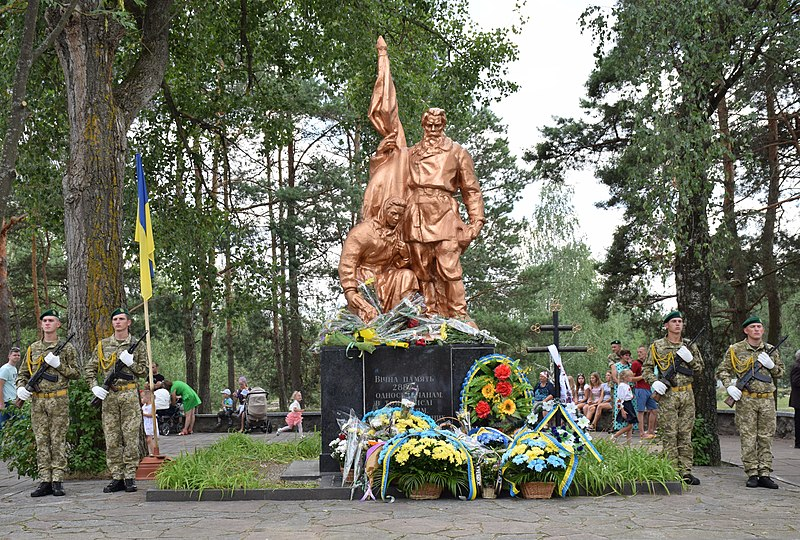
\includegraphics[width=0.8\linewidth]{0.jpg}
	
	\caption{\label{fig:frog3}Пам'ятник односельцям, загиблим в результаті трагедії 13 липня 1943 р.}
	
	\label{fig:mpr}
	
\end{figure}

\textbf{\textsl{13 липня 1941 року}} в село (вдерлися фашисти. Настали чорні дні неволі. Гітлерівці грабували населення, забирали хліб, худобу. 70 мирних жителів вивезли на каторжні роботи до Німеччини.

\textbf{13 липня 1943 року} в с.Копище сталася одна з найжахливіших трагедій України: нацистські загарбники влаштували \mbox{\textbf{\textsl{каральну операцію “Фрау Хельга” (пані Ольга)}}}, метою якої було повне знищення жителів села. \ref{fig:frog4} За один день спалили живими 2887 мирних жителів, з них 1347 дітей віком до 12 років. (Мал. \ref{fig:frog3})Врятувались лише четверо дорослих та 46 дітей.

Незважаючи на величезні труднощі, копищанці всі сили віддавали на відродження рідного села. Стало легше працювати, коли після перемоги над гітлерівською Німеччиною до села почали повертатися демобілізовані чоловіки.

Поступово піднімалося з руїн Копище. Вже через рік після перемоги тут виросла ціла вулиця. Один з будинків пристосували під лікарняний пункт, інший під початкову школу.

Основні сільськогосподарські культури у колгоспі — льон, картопля, зернові. Важливу роль у його економіці відіграє тваринництво м’ясо-молочного напряму. На 1 січня 1967 року колгосп мав 685 голів великої рогатої худоби, в т. ч. 275 корів та 199 голів овець. Для їх розміщення споруджено під шифером 5 добротних тваринницьких приміщень. На той час господарство було повністю електрифіковано, мало 9 тракторів, 6 комбайнів, 8 автомашин. Діяла пилорама.

На тваринницьких фермах обладнано автоматичне напування.

Копищанці справжні господарі своєї долі. 35 чоловік обрано депутатами сільської Ради, серед яких 15 жінок, 11 чоловік — членами правління колгоспу. В постійно діючих комісіях працює близько 100 чоловік. Бюджет Ради на 1973 рік становить 39 964 крб., переважна більшість цієї суми буде використана на поліпшення охорони здоров’я, на піднесення культурно-освітньої роботи.

В центрі Копища знаходиться Братьска могила жертвам фатишизму (1961 р.), в якій поховано 2887 жителів села, утому числі 1347 дітей (Мал. \ref{fig:frog3}).
\begin{figure}
	\centering
	\begin{subfigure}[b]{0.3\textwidth}
		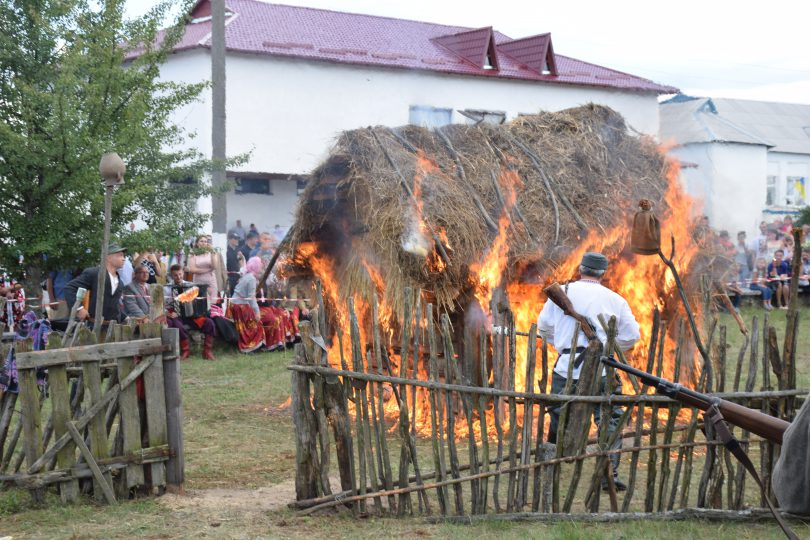
\includegraphics[width=\textwidth]{1.jpg}
		\caption{}
		\label{fig:gull}
	\end{subfigure}
	~ %add desired spacing between images, e. g. ~, \quad, \qquad, \hfill etc. 
	%(or a blank line to force the subfigure onto a new line)
	\begin{subfigure}[b]{0.3\textwidth}
		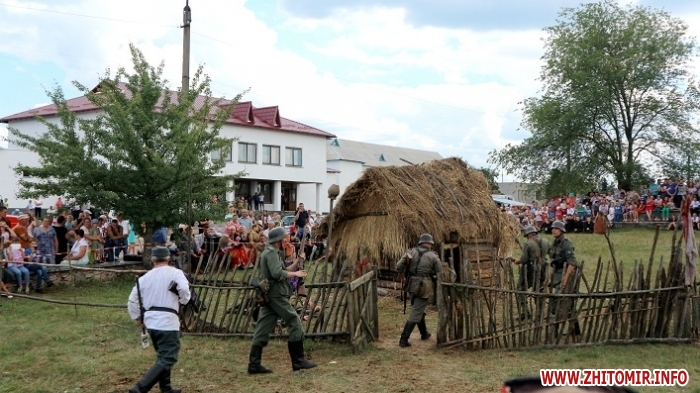
\includegraphics[width=\textwidth]{2.jpg}
		\caption{}
		\label{fig:tiger}
	\end{subfigure}
	~ %add desired spacing between images, e. g. ~, \quad, \qquad, \hfill etc. 
	%(or a blank line to force the subfigure onto a new line)
	\begin{subfigure}[b]{0.3\textwidth}
		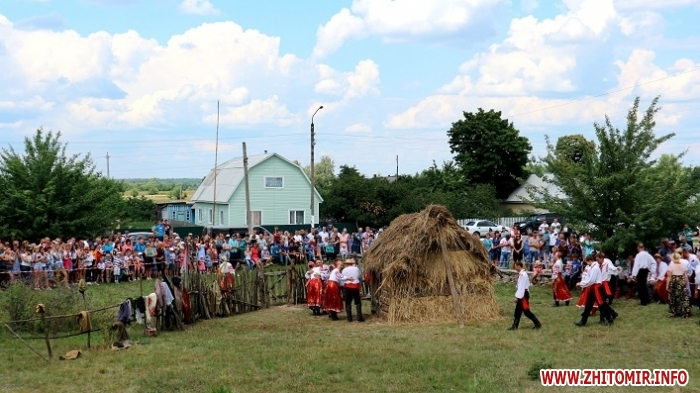
\includegraphics[width=\textwidth]{3.jpg}
		\caption{}
		\label{fig:mouse}
		\end{subfigure}
	\caption{\label{fig:frog4}Відзначення 75-ї річниці Копищенської трагедії}\label{fig:animals}
\end{figure}

Поруч знаходиться музей, який розповідає людям про історію рідного села і про страшну трагедію, яку не можна забути. Директор музею – Мартиновець Марія Василівна.

У селі наразі є загальноосвітня школа І-ІІІ ступенів.  Дітей навчається 200. Також функціонує заклад дошкільної освіти з короткотривалим перебуванням дітей без харчування, який відвідує 22 дітей.





